\documentclass[10pt]{article}
\usepackage[utf8]{inputenc}
\usepackage{graphicx}
\usepackage{wrapfig}
\usepackage{biblatex}



\title{Projeto e Implementação de Jogos 2D}
\author{Lorena Vilaça}
\date{21 de Outubro de 2019}


\addbibresource {lcjbv2.bib}
\begin{document}

\maketitle

\section{Introdução}    
\paragraph{} Nos últimos anos, vem crescendo o impacto dos aplicativos de entretenimento (conhecidos simplesmente como "jogos de computador") no mercado mundial de informática. Diante deste quadro e tendo em vista que já existe um esforço pernambucano pioneiro de pesquisa e desenvolvimento em jogos, tanto dentro do CIn-UFPE (Guararapes, Canyon, FutSim, Enigmas no Campus) quanto na iniciativa privada (JoyStudios, Jynx), a disciplina dá a oportunidade aos alunos de Ciência da Computação de se familiarizarem, em uma disciplina eletiva, com as técnicas, ferramentas e conceitos de projeto e implementação de jogos. Essa foi a primeira disciplina desse gênero no Brasil.

\begin{figure}[h!]
\centering
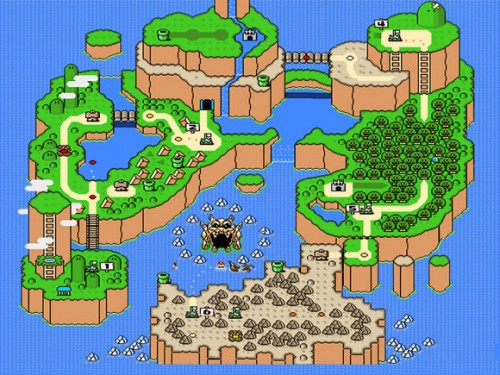
\includegraphics[width = 10cm]{marioworld.jpg} 
\caption {Mapa do Super Mario World (jogo 2D)}
\end{figure}


\section {Relevância} 
\paragraph{} A disciplina se baseia na criação de um jogo 2D, em grupos de estudantes. A partir do início do semestre há o auxilio para a construção do jogo, desde a ideia de qual jogo criar e de como funcionará, até a sua implementação, com esse jogo sendo apresentado e servindo de nota no final do período.
\paragraph{} Alguns dos livros utilizados são:
\begin{itemize}
    \item Game Programming Gems Series \cite {deloura2001game}
    \item Game Architecture and Design \cite {rollings1999game}
    \item Rules of Play: Game Design Fundamentals \cite {salen2004rules}
\end{itemize}
\paragraph{} Esse tipo de disciplina influencia no desenvolvimento da área de jogos em Pernambuco, que vem ganhando força através dos anos, permitindo que os alunos do CIn tenham um contato com o desenvolvimento de jogos e dando um conhecimento inicial de como funciona esse mundo.

\section {Relação com outras disciplinas}
\paragraph{} A cadeira tem algumas disciplinas como pré-requisito, que são:
\begin{itemize}
    \item IF680 - Processamento Gráfico
    \item IF684 - Sistemas Inteligentes
    \item IF687 - Introdução à multimídia
 \end{itemize}
\paragraph{} Os pré-requisitos são disciplinas que trabalham com a parte de construção gráfica, desenvolvimento de ambientes virtuais e aprendizagem de máquina, ferramentas necessárias para a criação de um jogo.


\printbibliography

\end{document}
